\documentclass[11pt]{article}

\usepackage{latexsym}
\usepackage{amssymb}
\usepackage{amsthm}
\usepackage{graphicx}
\usepackage{enumerate}
\usepackage{amsmath}
\usepackage{cancel}
\numberwithin{equation}{section}

\setlength{\evensidemargin}{.25in}
\setlength{\oddsidemargin}{-.25in}
\setlength{\topmargin}{-.75in}
\setlength{\textwidth}{6.5in}
\setlength{\textheight}{9.5in}
\newcommand{\due}{September 30th, 2015}
\newcommand{\HWnum}{4}
\newcommand{\grad}{\bold\nabla}
\newcommand{\vecE}{\vec{E}}
\newcommand{\scrptR}{\vec{\mathfrak{R}}}
\newcommand{\kapa}{\frac{1}{4\pi\epsilon_0}}
\newcommand{\emf}{\mathcal{E}}
\newcommand{\unit}[1]{\ensuremath{\, \mathrm{#1}}}
\newcommand{\real}{\textnormal{Re}}
\newcommand{\Erf}{\textnormal{Erf}}
\newcommand{\sech}{\textnormal{sech}}
\newcommand{\scrO}{\mathcal{O}}
\newcommand{\levi}{\widetilde{\epsilon}}
\newcommand{\partiald}[2]{\ensuremath{\frac{\partial{#1}}{\partial{#2}}}}
\newcommand{\norm}[2]{\langle{#1}|{#2}\rangle}
\newcommand{\inprod}[2]{\langle{#1}|{#2}\rangle}
\newcommand{\ket}[1]{|{#1}\rangle}
\newcommand{\bra}[1]{\langle{#1}|}





\begin{document}
\begin{titlepage}
\setlength{\topmargin}{1.5in}
\begin{center}
\Huge{Physics 3320} \\
\LARGE{Principles of Electricity and Magnetism II} \\
\Large{Professor Ana Maria Rey} \\[1cm]

\huge{Homework \#\HWnum}\\[0.5cm]

\large{Joe Becker} \\
\large{SID: 810-07-1484} \\
\large{\due} 

\end{center}

\end{titlepage}



\section{Problem \#1}
\begin{enumerate}[(a)]
\item For a point mass, $m$, sliding without friction inside a surface of revolution given 
by the rotation of $z=\alpha\sin(r/R)$ about the $\hat{z}$ axis. We see that this surface
creates a constrained motion where the motion in Cartesian coordinates including the 
constraints are
\begin{align*} 
x &= r\cos\theta\\
y &= r\sin\theta\\
z &= \alpha\sin(r/R)
\end{align*} 
we note that velocities associated with these coordinates is given by
\begin{align*}
\dot{x} &= \dot{r}\cos\theta-r\sin\theta\dot\theta\\
\dot{y} &= \dot{r}\sin\theta+r\cos\theta\dot\theta\\
\dot{z} &= \alpha\cos(r/R)\dot{r}/R
\end{align*}
Now we have converted to the generalized coordinates $r,\theta$ where we can write the 
kinetic energy in generalized coordinates as
\begin{align*}
T &= \frac{1}{2}m\left(\dot{x}^2+\dot{y}^2+\dot{z}^2\right)\\
&\Downarrow\\
T &= \frac{1}{2}m\left((\dot{r}\cos\theta-r\sin\theta\dot\theta)^2+(\dot{r}\sin\theta+r\cos\theta\dot\theta)^2+(\alpha\cos(r/R)\dot{r}/R)^2\right)\\
&= \frac{1}{2}m\left(\dot{r}^2\cos^2\theta + r^2\sin^2\theta\dot\theta^2 - \cancel{r\dot{r}\dot{\theta}\sin\theta\cos\theta} + \dot{r}^2\sin^2\theta + r^2\cos^2\theta\dot\theta^2 + \cancel{r\dot{r}\dot{\theta}\sin\theta\cos\theta} + \left(\frac{\alpha}{R}\right)^2\dot{r}^2\cos^2(r/R)\right)\\
&= \frac{1}{2}m\left(\dot{r}^2(\cos^2\theta+\sin^2\theta) + r^2\dot\theta^2(\sin^2\theta+\cos^2\theta) + \left(\frac{\alpha}{R}\right)^2\dot{r}^2\cos^2(r/R)\right)\\
&= \frac{1}{2}m\dot{r}^2\left(1+\left(\alpha/R\right)^2\cos^2(r/R)\right)+ \frac{1}{2}mr^2\dot\theta^2
\end{align*}
Next we can write the potential energy, $U$, in generalized coordinates by
\begin{align*}
U(z) &= mgz\\
&\Downarrow\\
U(r) &= mg\alpha\sin(r/R)
\end{align*}
Which gives us the \emph{Lagrangian} by
\begin{align*}
L &= T - U\\
&\Downarrow\\
L &= \frac{1}{2}m\dot{r}^2\left(1+\left(\alpha/R\right)^2\cos^2(r/R)\right)+ \frac{1}{2}mr^2\dot\theta^2 - mg\alpha\sin(r/R)
\end{align*}
Now we can use the \emph{Euler-Lagrange Equation} 
\begin{equation} 
\frac{\partial L}{\partial q_i} = \frac{d}{dt}\frac{\partial L}{\partial\dot{q}_i}
\label{EulerLag} 
\end{equation} 
for $q_i=r,\theta$. For $\theta$ we note that $L$ has no $\theta$ dependence this implies 
that the left hand side of equation \ref{EulerLag} is zero. Therefore
\begin{align*}
\frac{\partial L}{\partial\theta} &= \frac{d}{dt}\frac{\partial L}{\partial\dot{\theta}}\\
&\Downarrow\\
0 &= \frac{d}{dt}\frac{\partial}{\partial\dot{\theta}}\left(\frac{1}{2}mr^2\dot{\theta}^2\right)\\
0 &= \frac{d}{dt}\left(mr^2\dot{\theta}\right)
\end{align*}
We see that the time derivative of $mr^2\dot{\theta}$ is zero which implies that this 
quantity is conserved, which is the conservation of angular momentum, $l$,  which we can say
as
\begin{align*}
l &= mr^2\dot{\theta} \\
&\Downarrow\\
\dot{\theta} &= \frac{l}{mr^2}
\end{align*}
Next to calculate equation \ref{EulerLag} we first find
\begin{align*}
\frac{\partial L}{\partial r} &= \frac{\partial}{\partial r}\left(\frac{1}{2}m\dot{r}^2\left(1+\left(\alpha/R\right)^2\cos^2(r/R)\right)+ \frac{1}{2}mr^2\dot\theta^2 - mg\alpha\sin(r/R)\right)\\
&= \frac{1}{2}m\dot{r}^2\left(\alpha/R\right)^22\cos(r/R)(-\sin(r/R))\frac{1}{R} + mr\dot\theta^2 - mg\alpha/R\cos(r/R)\\
&= -\frac{\alpha^2}{R^3}m\dot{r}^2\cos(r/R)\sin(r/R) + \frac{l^2}{mr^3} - \frac{mg\alpha}{R}\cos(r/R)
\end{align*}
Next we need to calculate the $\dot{r}$ derivative by
\begin{align*}
\frac{\partial L}{\partial \dot{r}} &= \frac{\partial}{\partial\dot{r}}\left(\frac{1}{2}m\dot{r}^2\left(1+\left(\alpha/R\right)^2\cos^2(r/R)\right)+ \frac{1}{2}mr^2\dot\theta^2 - mg\alpha\sin(r/R)\right)\\
&= m\dot{r}\left(1+\left(\alpha/R\right)^2\cos^2(r/R)\right) 
\end{align*}
Then we can take the time derivative of the above term by
\begin{align*}
\frac{d}{dt}\frac{\partial L}{\partial \dot{r}} &= \frac{d}{dt}\left(m\dot{r}\left(1+\left(\alpha/R\right)^2\cos^2(r/R)\right)\right)\\
&= m\ddot{r} + m\ddot{r}\left(\alpha/R\right)^2\cos^2(r/R) + m\dot{r}\left(\alpha/R\right)^2(2\cos(r/R))(-\sin(r/R))\frac{\dot{r}}{R}\\
&= m\ddot{r} \left(1 + \left(\alpha/R\right)^2\cos^2(r/R)\right) - 2\frac{\alpha^2}{R^3}m\dot{r}^2\cos(r/R)\sin(r/R)
\end{align*}
Now we can write equation \ref{EulerLag} as
\begin{align*}
\frac{\partial L}{\partial r} &= \frac{d}{dt}\frac{\partial L}{\partial\dot{r}}\\
&\Downarrow\\
-\frac{\alpha^2}{R^3}m\dot{r}^2\cos(r/R)\sin(r/R) + \frac{l^2}{mr^3} - \frac{mg\alpha}{R}\cos(r/R) &= m\ddot{r} \left(1 + \left(\alpha/R\right)^2\cos^2(r/R)\right) - 2\frac{\alpha^2}{R^3}m\dot{r}^2\cos(r/R)\sin(r/R)\\
\frac{\alpha^2}{R^3}\dot{r}^2\cos(r/R)\sin(r/R) + \frac{l^2}{m^2r^3} - \frac{g\alpha}{R}\cos(r/R) &= \ddot{r} \left(1 + \left(\alpha/R\right)^2\cos^2(r/R)\right)
\end{align*}
So we have the equation of motion
$$\ddot{r} = \frac{1}{\left(1 + \left(\alpha/R\right)^2\cos^2(r/R)\right)}\left(\frac{\alpha^2}{R^3}\dot{r}^2\cos(r/R)\sin(r/R) + \frac{l^2}{m^2r^3} - \frac{g\alpha}{R}\cos(r/R)\right)$$

\item
We can use the result from part (b) to determine if there exists a stationary horizontal
circular orbits by noting that a stationary horizontal circular orbit implies that $z$ 
remains constant which implies that $r$ remains constant because it is constrained by 
$z=\alpha\cos(r/R)$. So for $r=r_0$ we see that $\dot{r}=\ddot{r}$ which makes the equation of 
motion in $\theta$ becomes
\begin{align*}
\dot{\theta} &= \frac{l}{mr_0^2}
\end{align*}
which we can see is constant for horizontal orbital motion. Therefore we can define an 
angular frequency, $\omega_0$, as
\begin{equation}
\omega_0 \equiv \frac{l}{mr_0^2}.
\label{omega0}
\end{equation}
Therefore we can change our equation of motion for $r$ using these two results as
\begin{align*}
0 &= \frac{1}{\left(1 + \left(\alpha/R\right)^2\cos^2(r_0/R)\right)}\left(\frac{l^2}{m^2r_0^3} - \frac{g\alpha}{R}\cos(r_0/R)\right)\\
0 &= \omega_0^2r_0 - \frac{g\alpha}{R}\cos(r_0/R)\\
&\Downarrow\\
\omega_0^2 &= \frac{g\alpha}{Rr_0}\cos(r_0/R)
\end{align*}
We see that for any $r_0$ in $0<r_0<(\pi/2)R$ we have an $\omega_0$ this implies that we can
have stationary horizontal circular orbits.

\item Now we can test the stability of these orbits by taking a small perturbation in the 
form of $r\rightarrow r_0+\delta r$ and expand into first order in $\delta r$. We note that 
for this perturbative $r$ we have $\dot{r} = \delta\dot{r}$ and $\ddot{r} = \delta\ddot{r}$.
Next we can expand the trigonometric functions using the assumption that $\delta r$ is 
small. First for sine we have
\begin{align*}
\sin\left(\frac{r_0}{R}+\frac{\delta r}{R}\right) &= \sin\left(\frac{r_0}{R}\right)\cancelto{1}{\cos\left(\frac{\delta r}{R}\right)} + \cos\left(\frac{r_0}{R}\right)\cancelto{\delta r/R}{\sin\left(\frac{\delta r}{R}\right)}\\
&= \sin\left(\frac{r_0}{R}\right) + \frac{\delta r}{R}\cos\left(\frac{r_0}{R}\right)
\end{align*}
and for cosine we have
\begin{align*}
\cos\left(\frac{r_0}{R}+\frac{\delta r}{R}\right) &= \cos\left(\frac{r_0}{R}\right)\cancelto{1}{\cos\left(\frac{\delta r}{R}\right)} - \sin\left(\frac{r_0}{R}\right)\cancelto{\delta r/R}{\sin\left(\frac{\delta r}{R}\right)}\\
&= \cos\left(\frac{r_0}{R}\right) - \frac{\delta r}{R}\sin\left(\frac{r_0}{R}\right)
\end{align*}
Using the above expansion we can expand to first order in $\delta r$ the terms
\begin{align*}
\cos^2\left(\frac{r_0}{R}+\frac{\delta r}{R}\right) &=  \left(\cos\left(\frac{r_0}{R}\right) - \frac{\delta r}{R}\sin\left(\frac{r_0}{R}\right)\right)^2\\
&=  \cos^2\left(\frac{r_0}{R}\right) - 2\frac{\delta r}{R}\sin\left(\frac{r_0}{R}\right)\cos\left(\frac{r_0}{R}\right) + \scrO(\delta r^2)\\
&=  \cos^2\left(\frac{r_0}{R}\right) - \frac{\delta r}{R}\sin\left(2\frac{r_0}{R}\right)
\end{align*}
We note that the $\dot{r}^2$ term becomes $\delta\dot{r}^2$ which is second order in 
$\delta{r}$ so we can neglect this term. This implies that our equations of motion become
\begin{align*}
\ddot{r} &= \frac{1}{\left(1 + \left(\alpha/R\right)^2\cos^2(r/R)\right)}\left(\frac{\alpha^2}{R^3}\dot{r}^2\cos(r/R)\sin(r/R) + \frac{l^2}{m^2r^3} - \frac{g\alpha}{R}\cos(r/R)\right)\\
&\Downarrow\\
\delta\ddot{r} &= \frac{1}{\left(1 + \left(\alpha/R\right)^2\cos^2((r_0+\delta{r})/R)\right)}\left(\frac{l^2}{m^2(r_0+\delta{r})^3} - \frac{g\alpha}{R}\cos((r_0+\delta{r})/R))\right)\\
&= \frac{1}{\left(1 + \left(\alpha/R\right)^2\left(\cos^2(r_0/R)-\frac{\delta{r}}{R}\sin(2r_0/R)\right)\right)}\left(\frac{l^2}{m^2(r_0^3+3r_0^2\delta{r})} - \frac{g\alpha}{R}\cos(r_0/R) + \frac{g\alpha\delta{r}}{R^2}\sin(r_0/R)\right)
\end{align*}
We now note the result from stationary horizontal circular orbit 
$$\omega_0 = \frac{l}{mr_0^2},\qquad \cos(r_0/R)=\frac{\omega_0Rr_0}{g\alpha}$$
which we replace into the equation of motion as
\begin{align*}
\delta\ddot{r} &= \frac{1}{\left(1 + \left(\alpha/R\right)^2\left(\left(\frac{\omega_0Rr_0}{a\alpha}\right)^2-\frac{\delta{r}}{R}\sin(2r_0/R)\right)\right)}\left(\frac{l^2}{m^2r_0^4(\frac{1}{r_0}+\frac{3r_0^2\delta{r}}{r_0^4})} - \frac{g\alpha}{R}\frac{\omega_0^2Rr_0}{g\alpha} + \frac{g\alpha\delta{r}}{R^2}\sin(r_0/R)\right)\\
&= \frac{1}{\left(1 + \left(\frac{\omega_0^2r_0}{g}\right)^2-\frac{\alpha^2\delta{r}}{R^3}\sin(2r_0/R)\right)}\left(\frac{\omega_0^2}{\frac{1}{r_0}+\frac{3\delta{r}}{r_0^2}} - \omega_0^2r_0 + \frac{g\alpha\delta{r}}{R^2}\sin(r_0/R)\right)\\
&= \frac{1}{\left(1 + \left(\frac{\omega_0^2r_0}{g}\right)^2-\frac{\alpha^2\delta{r}}{R^3}\sin(2r_0/R)\right)}\left(\frac{\omega_0^2r_0}{1+3\delta{r}/r_0} - \omega_0^2r_0 + \frac{g\alpha\delta{r}}{R^2}\sin(r_0/R)\right)
\end{align*}
We note that we can expand 
$$\frac{1}{1+3\delta{r}/r_0} = 1 - 3\frac{\delta{r}}{r_0} + \scrO(\delta{r}^2)$$
for a small $\delta{r}$. Also, we can see that if we move the fractional pre-factor over to
the left hand side we get 
$$\delta\ddot{r}\left(1+ \left(\frac{\omega_0^2r_0}{g}\right)^2\right)-\delta\ddot{r}\delta{r}\frac{\alpha^2}{R^3}\sin(2r_0/R)$$
the term $\delta\ddot{r}\delta{r}\frac{\alpha^2}{R^3}\sin(2r_0/R)$ is of second order in 
$\delta{r}$ so we can neglect the term which makes the equation of motion become
\begin{align*}
\delta\ddot{r} &= \frac{1}{1 + \left(\frac{\omega_0^2r_0}{g}\right)^2}\left(\omega_0^2r_0\left(1-\frac{3\delta{r}}{r_0} - 1\right) + \frac{g\alpha\delta{r}}{R^2}\sin(r_0/R)\right)\\
&= \frac{g^2}{g^2 + (\omega_0r_0)^2}\left(-3\omega_0^2\delta{r} + \frac{g\alpha\delta{r}}{R^2}\sin(r_0/R)\right)\\
&= \frac{g^2}{g^2 + (\omega_0r_0)^2}\left(\frac{g\alpha}{R^2}\sin(r_0/R)-3\omega_0^2\right)\delta{r}\\
\end{align*}
We see that we have a differential equation in the form of simple oscillatory motion given 
by
$$\ddot{q} = -kq.$$
We note that the condition for stable circular motion is when
$$\frac{g^2}{g^2 + (\omega_0r_0)^2}\left(\frac{g\alpha}{R^2}\sin(r_0/R)-3\omega_0^2\right)>0$$
which can be reduced to a condition on $\omega_0$ by
\begin{align*}
\cancel{\frac{g^2}{g^2 + (\omega_0r_0)^2}}\left(\frac{g\alpha}{R^2}\sin(r_0/R)-3\omega_0^2\right) &> 0\\
&\Downarrow\\
\frac{g\alpha}{3R^2}\sin(r_0/R) &> \omega_0^2
\end{align*}

\item
The result from part (c) for a small perturbation $\delta{r}$ we have oscillations about 
circular orbit given by
$$\delta\ddot{r} = \Omega^2\delta{r}$$
where
$$\Omega^2\equiv\frac{g^2}{g^2 + (\omega_0r_0)^2}\left(\frac{g\alpha}{R^2}\sin(r_0/R)-3\omega_0^2\right)$$
under the condition 
$$\omega_0^2 < \frac{g\alpha}{3R^2}\sin(r_0/R)$$
which makes $\Omega$ negative. Therefore for a small deviation from the circular orbit a 
point mass can perform harmonic oscillations with a frequency of 
$$\Omega = \sqrt{\frac{g^2}{g^2 + (\omega_0r_0)^2}\left(\frac{g\alpha}{R^2}\sin(r_0/R)-3\omega_0^2\right)}$$
\end{enumerate}

\pagebreak

\section{Problem \#2}
\begin{enumerate}[(a)]
\item For a point mass, $m$, sliding without friction inside a surface of revolution given 
by the rotation of $z=\alpha\left(1-e^{r/R}\right)$ about the $\hat{z}$ axis. We see that this surface
creates a constrained motion where the motion in Cartesian coordinates including the 
constraints are
\begin{align*} 
x &= r\cos\theta\\
y &= r\sin\theta\\
z &= \alpha\left(1-e^{r/R}\right)
\end{align*} 
we note that velocities associated with these coordinates is given by
\begin{align*}
\dot{x} &= \dot{r}\cos\theta-r\sin\theta\dot\theta\\
\dot{y} &= \dot{r}\sin\theta+r\cos\theta\dot\theta\\
\dot{z} &= \frac{\alpha}{R}e^{-r/R}\dot{r}
\end{align*}
Like before we calculate the kinetic energy in the generalized coordinates $r,\theta$ by
\begin{align*}
T &= \frac{1}{2}m\left(\dot{x}^2 + \dot{y}^2 + \dot{z}^2\right)\\
&= \frac{1}{2}m\left((\dot{r}\cos\theta-r\sin\theta\dot\theta)^2 + (\dot{r}\sin\theta+r\cos\theta\dot\theta)^2 + \left(\frac{\alpha}{R}e^{-r/R}\dot{r}\right)^2\right)\\
&= \frac{1}{2}m\left(\dot{r}^2 + r^2\dot{\theta}^2 + \frac{\alpha^2}{R^2}e^{-2r/R}\dot{r}^2\right)\\
&= \frac{1}{2}m\dot{r}^2 \left(1 + \frac{\alpha^2}{R^2}e^{-2r/R}\right) + \frac{1}{2}mr^2\dot{\theta}^2 
\end{align*}
Next we write the potential energy in $r,\theta$ as
$$U = mgz = mg\alpha\left(1-e^{-r/R}\right)$$
Therefore our Lagrangian is given by
$$L =\frac{1}{2}m\dot{r}^2 \left(1 + \frac{\alpha^2}{R^2}e^{-2r/R}\right) + \frac{1}{2}mr^2\dot{\theta}^2 - mg\alpha\left(1-e^{-r/R}\right)$$
Which we will use in equation \ref{EulerLag}. We note that the same conservation of angular
momentum condition from problem 1 in by the application of equation \ref{EulerLag} in the 
$\theta$ component
$$\dot{\theta} = \frac{l}{mr^2}$$
Next we can solve for the equation of motion for the $r$ coordinate, first we calculate
\begin{align*}
\partiald{L}{r} &= \partiald{}{r}\left(\frac{1}{2}m\dot{r}^2 \left(1 + \frac{\alpha^2}{R^2}e^{-2r/R}\right) + \frac{1}{2}mr^2\dot{\theta}^2 - mg\alpha\left(1-e^{-r/R}\right)\right)\\
&= \frac{1}{2}m\dot{r}^2\frac{\alpha^2}{R^2}e^{-2r/R}(-2/R) + mr\dot{\theta}^2 - mg\alpha\left(-e^{-r/R}\right)(-1/R)\\
&= -m\dot{r}^2\frac{\alpha^2}{R^3}e^{-2r/R} + \frac{l^2}{mr^3} - \frac{mg}{R}\alpha e^{-r/R}
\end{align*}
Next we calculate the $\dot{r}$ derivatives
\begin{align*}
\frac{d}{dt}\left(\partiald{L}{\dot{r}}\right) &= \frac{d}{dt}\left[\partiald{}{\dot{r}}\left(\frac{1}{2}m\dot{r}^2 \left(1 + \frac{\alpha^2}{R^2}e^{-2r/R}\right) + \frac{1}{2}mr^2\dot{\theta}^2 - mg\alpha\left(1-e^{-r/R}\right)\right)\right]\\
&= \frac{d}{dt}\left[m\dot{r}\left(1 + \frac{\alpha^2}{R^2}e^{-2r/R}\right)\right]\\  
&= m\ddot{r} + \frac{d}{dt}\left[m\dot{r}\frac{\alpha^2}{R^2}e^{-2r/R}\right]\\  
&= m\ddot{r} + m\ddot{r}\frac{\alpha^2}{R^2}e^{-2r/R}+ m\dot{r}\frac{\alpha^2}{R^2}e^{-2r/R}(-2\dot{r}/R)\\
&= m\ddot{r} + m\ddot{r}\frac{\alpha^2}{R^2}e^{-2r/R} - 2m\dot{r}^2\frac{\alpha^2}{R^3}e^{-2r/R}
\end{align*}
Now we can write the full equation \ref{EulerLag} and solve the equation of motion for the 
$r$ coordinate as
\begin{align*}
m\ddot{r} + m\ddot{r}\frac{\alpha^2}{R^2}e^{-2r/R} - 2m\dot{r}^2\frac{\alpha^2}{R^3}e^{-2r/R} &= -m\dot{r}^2\frac{\alpha^2}{R^3}e^{-2r/R} + \frac{l^2}{mr^3} - \frac{mg}{R}\alpha e^{-r/R}\\
m\ddot{r}\left(1 + \frac{\alpha^2}{R^2}e^{-2r/R}\right)  &= m\dot{r}^2\frac{\alpha^2}{R^3}e^{-2r/R} + \frac{l^2}{mr^3} - \frac{mg}{R}\alpha e^{-r/R}\\
\ddot{r}\left(1 + \frac{\alpha^2}{R^2}e^{-2r/R}\right)  &= \dot{r}^2\frac{\alpha^2}{R^3}e^{-2r/R} + \frac{l^2}{m^2r^3} - \frac{g}{R}\alpha e^{-r/R}\\
\ddot{r} &= \left(1 + \frac{\alpha^2}{R^2}e^{-2r/R}\right)^{-1}\left(\dot{r}^2\frac{\alpha^2}{R^3}e^{-2r/R} + \frac{l^2}{m^2r^3} - \frac{g}{R}\alpha e^{-r/R}\right)
\end{align*}

\item We can take the equation of motion that we found in part (b) to see if there exists
a stationary horizontal circular orbit by applying the condition $r=r_0$ where $r_0$ is a
constant. This again implies that $\ddot{r}=\dot{r}=0$. This makes the equation of motion 
become
\begin{align*}
\cancelto{0}{\ddot{r}} &= \left(1 + \frac{\alpha^2}{R^2}e^{-2r_0/R}\right)^{-1}\left(\cancelto{0}{\dot{r}^2\frac{\alpha^2}{R^3}e^{-2r_0/R}} + \frac{l^2}{m^2r_0^3} - \frac{g}{R}\alpha e^{-r_0/R}\right)\\
&= \cancel{\left(1 + \frac{\alpha^2}{R^2}e^{-2r_0/R}\right)^{-1}}\left(\frac{l^2}{m^2r_0^3} - \frac{g}{R}\alpha e^{-r_0/R}\right)\\
&= \frac{l^2}{m^2r_0^3} - \frac{g}{R}\alpha e^{-r_0/R}\\
\frac{l^2}{m^2r_0^3} &= \frac{g}{R}\alpha e^{-r_0/R}\\
&\Downarrow\\
\omega_0^2r_0 &= \frac{g}{R}\alpha e^{-r_0/R}\\
\omega_0^2 &= \frac{g\alpha}{Rr_0}e^{-r_0/R}
\end{align*}
Note that we used the definition of $\omega_0$ from equation \ref{omega0}. We note that there
exists an angular frequency, $\omega_0$, for stationary horizontal circular orbits. We see 
that for $0 < r_0$ there is an $\omega_0$ that exists.  

\item For the stationary horizontal circular orbits found in part (b) we can test if the 
orbits are stable by adding a perturbation $\delta r$ to the radius of stationary horizontal
circular orbits, $r_0$. So we take our equation of motion and apply $r\rightarrow r_0+
\delta{r}$ and expand to first order in $\delta{r}$. We can see that we expand
\begin{align*}
\exp\left(-\frac{2(r_0+\delta{r})}{R}\right) &= \exp\left(-\frac{2r_0}{R}\right)\exp\left(-\frac{2\delta{r}}{R}\right)\\
&= \exp\left(-\frac{2r_0}{R}\right)\left(1-\frac{2\delta{r}}{R} + \scrO(\delta{r}^2)\right)\\
&= e^{-2r_0/R} - 2\frac{\delta{r}}{R} e^{-2r_0/R}
\end{align*}
and
\begin{align*}
\exp\left(-\frac{r_0+\delta{r}}{R}\right) &= \exp\left(-\frac{r_0}{R}\right)\exp\left(-\frac{\delta{r}}{R}\right)\\
&= \exp\left(-\frac{r_0}{R}\right)\left(1-\frac{1}{2}\frac{\delta{r}}{R} + \scrO(\delta{r}^2)\right)\\
&= e^{-r_0/R} - \frac{\delta{r}}{R} e^{-r_0/R}
\end{align*}
We also expand the angular momentum term as
\begin{align*}
\frac{l^2}{m^2(r_0+\delta{r})^3} &=  \frac{l^2}{m^2(r_0^3+3r_0^2\delta{r}+\scrO(\delta{r}^2))}\\
&=  \frac{l^2}{m^2r_0^3\left(\frac{1}+3\frac{\delta{r}}{r_0}\right)}\\
&=  \frac{l^2}{m^2r_0^3}\left(1 - 3\frac{\delta{r}}{r_0} + \scrO(\delta{r}^2)\right)
\end{align*}
So we use these expansions and see that equation of motion becomes
\begin{align*}
\ddot{r} &= \left(1 + \frac{\alpha^2}{R^2}e^{-2r/R}\right)^{-1}\left(\dot{r}^2\frac{\alpha^2}{R^3}e^{-2r/R} + \frac{l^2}{m^2r^3} - \frac{g}{R}\alpha e^{-r/R}\right)\\
&\Downarrow\\
\delta\ddot{r}\left(1 + \frac{\alpha^2}{R^2}e^{-2(r_0+\delta{r})/R}\right) &= \cancelto{\delta{r}^2}{\delta\dot{r}^2\frac{\alpha^2}{R^3}e^{-2(r_0+\delta{r})/R}} + \frac{l^2}{m^2(r_0+\delta{r})^3} - \frac{g}{R}\alpha e^{-(r_0+\delta{r})/R}\\
&\Downarrow\\
\delta\ddot{r} + \delta\ddot{r}\frac{\alpha^2}{R^2}\left(e^{-2r_0/R} - \cancelto{\delta{r}^2}{2\frac{\delta{r}}{R}e^{-2r_0/R}}\right) &= \frac{l^2}{m^2r_0^3}\left(1 -3\frac{\delta{r}}{r_0}\right)  - \frac{g\alpha}{R}\left(e^{-r_0/R}-\frac{\delta{r}}{R}e^{-r_0/R}\right)\\
\delta\ddot{r}\left(1 + \frac{\alpha^2}{R^2}e^{-2r_0/R}\right) &= \frac{l^2}{m^2r_0^3}\left(1 -3\frac{\delta{r}}{r_0}\right)  - \frac{g\alpha}{R}\left(e^{-r_0/R}-\frac{\delta{r}}{R}e^{-r_0/R}\right)
\end{align*}
We also need to use the result from a stable horizontal circular orbit given by
$$\omega_0 = \frac{l}{mr_0^2},\qquad e^{-r_0/R} = \frac{\omega_0^2r_0R}{g\alpha}$$
we can replace these terms by
\begin{align*}
\delta\ddot{r}\left(1 + \frac{\alpha^2}{R^2}e^{-2r_0/R}\right) &= \frac{l^2}{m^2r_0^3}\left(1 -3\frac{\delta{r}}{r_0}\right)  - \frac{g\alpha}{R}\left(e^{-r_0/R}-\frac{\delta{r}}{R}e^{-r_0/R}\right)\\
\delta\ddot{r}\left(1 + \frac{\alpha^2}{R^2}\left(e^{-r_0/R}\right)^2\right) &= \omega_0^2r_0\left(1 -3\frac{\delta{r}}{r_0}\right)  - \frac{g\alpha}{R}e^{-r_0/R}\left(1-\frac{\delta{r}}{R}\right)\\
&\Downarrow\\
\delta\ddot{r}\left(1 + \frac{\alpha^2}{R^2}\left(\frac{\omega_0^2r_0R}{g\alpha}\right)^2\right) &= \omega_0^2r_0\left(1 -3\frac{\delta{r}}{r_0}\right)  - \frac{g\alpha}{R}\frac{\omega_0^2r_0R}{g\alpha}\left(1-\frac{\delta{r}}{R}\right)\\
\delta\ddot{r}\left(1 + \left(\frac{\omega_0^2r_0}{g}\right)^2\right) &= \omega_0^2r_0\left(1 -3\frac{\delta{r}}{r_0}\right)  - \omega_0^2r_0\left(1-\frac{\delta{r}}{R}\right)\\
\delta\ddot{r}\left(\frac{g^2 + (\omega_0^2r_0)^2}{g^2}\right) &= \cancel{\omega_0^2r_0} - 3\omega_0^2r_0\frac{\delta{r}}{r_0} - \cancel{\omega_0^2r_0} + \omega_0^2r_0\frac{\delta{r}}{R}\\
\delta\ddot{r}\left(\frac{g^2 + (\omega_0^2r_0)^2}{g^2}\right) &=  \omega_0^2r_0\left(\frac{1}{R} - \frac{3}{r_0}\right)\delta{r}\\
\delta\ddot{r} &= \frac{g^2}{g^2 + (\omega_0^2r_0)^2} \omega_0^2r_0\frac{r_0-3R}{Rr_0}\delta{r}\\
\delta\ddot{r} &= \left(\frac{g^2\omega_0^2}{g^2 + (\omega_0^2r_0)^2}\frac{r_0-3R}{R}\right)\delta{r}
\end{align*}
Again we have an equation for harmonic motion in $\delta{r}$ again for these orbits to be
stable we need the condition that the pre-factor to $\delta{r}$ be negative. We can see that
for this condition to met we need to have $r_0 - 3R<0$ the is due to the fact that every 
other term can only be positive. So only circular orbits with radius $r_0<3R$ are stable. 
We also note that we require that there must be a non-zero angular velocity $\omega_0$.

\item As we found in part (c) for small perturbations we have stable orbits for the 
condition $r_0<6R$. We also see that the equation of motion is of the form 
$$\delta\ddot{r} = \Omega'^2\delta{r}$$
where
$$\Omega'^2\equiv\frac{g^2\omega_0^2}{g^2 + (\omega_0^2r_0)^2}\frac{r_0-3R}{R}$$
This corresponds to harmonic oscillations about a stable horizontal circular orbit with a 
oscillation frequency $\Omega'$.
\end{enumerate}

\pagebreak

\section{Problem \#3}
\begin{enumerate}[(a)]
\item We can derive generalized coordinates for a cycloid by looking at a circle of radius 
$a$ rolling below the $x$ axis. If we take a circle to have rolled an angle $\theta$ we can 
see that it moves an arc length, $a\theta$. The geometry of this is shown in Figure 
\ref{Figure}.
\begin{figure}
\centering
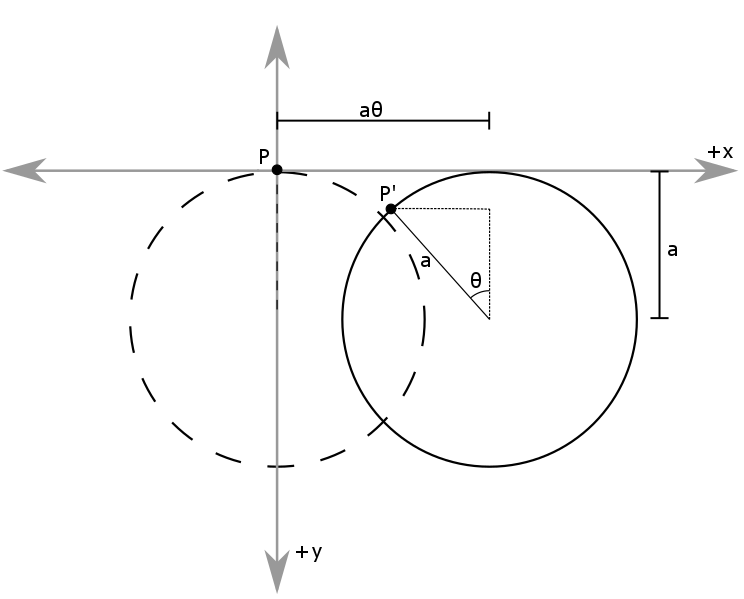
\includegraphics[width=1.0\textwidth]{Figure.png}
\caption{A circle rolling an angle $\theta$ below the $x$ axes, where point $P$ traces out 
a cycloid.}
\label{Figure}
\end{figure}
Now, we can look at point $P' = (x,y)$ in Figure \ref{Figure} we can see that it is a distance 
$a\sin\theta$ behind the center of the circle which is at a distance $a\theta$ from the 
start. So the distance moved in the $x$ direction is given by
$$x = a\theta - a\sin\theta = a(\theta-\sin\theta).$$
Next, we see that the height of point $P'$ is $a\cos\theta$ from the center of the circle
which is the radius, $a$, this implies that the $y$ coordinate is given by
$$y = a - a\cos\theta = a(1-\cos\theta).$$
We note that the distance the particle travels along the path of the cycloid by taking a 
path integral from 
$$s = \int_{0}^{\theta}\sqrt{\left(\frac{dx}{d\theta'}\right)^2 + \left(\frac{dy}{d\theta'}\right)^2}d\theta'$$
where we note that
\begin{align*}
\frac{dx}{d\theta} &= a(1-\cos\theta)\\
\frac{dx}{d\theta} &= a\sin\theta
\end{align*}
In order to calculate the distance from the minimum of the cycloid we note that the minimum
is when $\theta = \pi$ so we integrate from $\pi$.
\begin{align*}
s &= \int_{\pi}^{\theta}\sqrt{\left(\frac{dx}{d\theta'}\right)^2 + \left(\frac{dy}{d\theta'}\right)^2}d\theta'\\
&= \int_{\pi}^{\theta}\sqrt{\left(a(1-\cos\theta')\right)^2 + \left(a\sin\theta'\right)^2}d\theta'\\
&= \int_{\pi}^{\theta}\sqrt{a^2-2a^2\cos\theta'+a^2\cos^2\theta'+a^2\sin^2\theta'}d\theta'\\
&= \int_{\pi}^{\theta}\sqrt{2a^2-2a^2\cos\theta'}d\theta'\\
&= a\int_{\pi}^{\theta}\sqrt{2(1-\cos\theta')}d\theta'\\
&= a\int_{\pi}^{\theta}\sqrt{2(2\sin^2(\theta'/2))}d\theta'\\
&= -4a\left.\cos(\theta'/2)\right|_{\pi}^{\theta}\\
&= -4a\cos(\theta/2)
\end{align*}

\item For a mass that is constrained by this cycloid in a gravitational field given by
$g\hat{y}$ which we note points down because we defined the positive $y$ direction as 
down. We can use the result to gain our generalized coordinate $\theta$
\begin{align*}
x &=  a(\theta-\sin\theta)\\
y &=  a(1-\cos\theta)
\end{align*}
where
\begin{align*}
\dot{x} &=  a(\dot{\theta}-\cos\theta\dot{\theta}) =  a\dot{\theta}(1-\cos\theta)\\
\dot{y} &=  a\sin\theta\dot{\theta} 
\end{align*}
So in order to find the equations of motion we first construct the Lagrangian by noting that
the potential energy is
$$U = -mgy = -mga(1-\cos\theta)$$
and we can calculate the kinetic energy by
\begin{align*}
T &= \frac{1}{2}m\left(\dot{x}^2+\dot{y}^2\right)\\
&= \frac{1}{2}m\left((a\dot{\theta}(1-\cos\theta))^2+(a\sin\theta\dot{\theta})^2\right)\\
&= \frac{1}{2}m\left(a^2\dot{\theta}^2(1-2\cos\theta+\cos^2\theta)+a^2\dot{\theta}^2\sin^2\theta\right)\\
&= \frac{1}{2}ma^2\dot{\theta}^2\left(1-2\cos\theta+\cos^2\theta+\sin^2\theta\right)\\
&= ma^2\dot{\theta}^2\left(1-\cos\theta\right)
\end{align*}
Therefore we can write our Lagrangian as
$$L = ma^2\dot{\theta}^2\left(1-\cos\theta\right) + mga(1-\cos\theta)$$
Next we can find the equation of motion in the generalized coordinate, $\theta$, by equation
\ref{EulerLag}. First we find
\begin{align*}
\partiald{L}{\theta} &= \partiald{}{\theta}\left(ma^2\dot{\theta}^2\left(1-\cos\theta\right) + mga(1-\cos\theta)\right)\\
&= ma^2\dot{\theta}^2\left(-(-\sin\theta)\right) + mga(-(-\sin\theta))\\
&= ma\sin\theta(a\dot{\theta}^2+g)
\end{align*}
Then we find
\begin{align*}
\frac{d}{dt}\partiald{L}{\dot{\theta}} &= \frac{d}{dt}\left[\partiald{}{\dot{\theta}}\left(ma^2\dot{\theta}^2\left(1-\cos\theta\right) + mga(1-\cos\theta)\right)\right]\\
&= \frac{d}{dt}\left[2ma^2\dot{\theta}\left(1-\cos\theta\right)\right]\\
&= 2ma^2\ddot{\theta} - \frac{d}{dt}\left[2ma^2\dot{\theta}\cos\theta\right]\\
&= 2ma^2\ddot{\theta} - 2ma^2\ddot{\theta}\cos\theta - 2ma^2\dot{\theta}(-\sin\theta)\dot{\theta}\\
&= 2ma^2\ddot{\theta}(1 - \cos\theta) + 2ma^2\dot{\theta}^2\sin\theta
\end{align*}
So, equation \ref{EulerLag} becomes
\begin{align*}
2ma^2\ddot{\theta}(1 - \cos\theta) + 2ma^2\dot{\theta}^2\sin\theta &= ma\sin\theta(a\dot{\theta}^2+g)\\
2ma^2\ddot{\theta}(1 - \cos\theta) &= ma\sin\theta(a\dot{\theta}^2+g) - 2ma^2\dot{\theta}^2\sin\theta \\
\ddot{\theta}(1 - \cos\theta) &= \frac{ma}{2ma^2}\sin\theta(a\dot{\theta}^2+g-2a\dot{\theta}^2)\\ 
\ddot{\theta} &= \frac{1}{2}\frac{\sin\theta}{1-\cos\theta}\left(\frac{g}{a}-\dot{\theta}^2\right)\\
\ddot{\theta} &= \frac{1}{2}\frac{2\sin\theta/2\cos\theta/2}{2\sin^2\theta/2}\left(\frac{g}{a}-\dot{\theta}^2\right)\\
\ddot{\theta} &= \frac{\cot(\theta/2)}{2}\left(\frac{g}{a}-\dot{\theta}^2\right)
\end{align*}
In order to solve the equation of motion as a function of the position on the cycloid $s(t)$
we need to note the result from part (a) and get $\theta$ as a function of $s$
\begin{align*}
s &= -4a\cos(\theta/2)\\
&\Downarrow\\
\theta(s) &= 2\arccos\left(-\frac{s}{4a}\right)
\end{align*}
Where we calculate the first and second derivative noting that $d_x\arccos(x) = -(1-x^2)^{-1/2}$
which yields
\begin{align*}
\dot{\theta}(s) &= -2\frac{1}{\sqrt{1-(s/4a)^2}}(-\dot{s}/4a)\\
&= \frac{2\dot{s}}{4a}\frac{1}{\sqrt{1-(s/4a)^2}}\\
&= \frac{2\dot{s}}{4a}\frac{4a}{\sqrt{16a^2-s^2}}\\
&= \frac{2\dot{s}}{\sqrt{16a^2-s^2}}
\end{align*}
and
\begin{align*}
\ddot{\theta}(s) &= \frac{2\ddot{s}}{\sqrt{16a^2-s^2}} + 2\dot{s}\frac{d}{dt}\left[\frac{}{}(16a^2-s^2)^{-1/2}\right]\\
&= \frac{2\ddot{s}}{\sqrt{16a^2-s^2}} + 2\dot{s}(-1/2)(16a^2-s^2)^{-3/2}(-2s\dot{s})\\
&= \frac{2\ddot{s}}{\sqrt{16a^2-s^2}} + \frac{2s\dot{s}^2}{(16a^2-s^2)^{3/2}}
\end{align*}
We also calculate 
\begin{align*}
\cot(\theta/2) &= \cot\left(\frac{1}{2}2\arccos\left(\frac{-s}{4a}\right)\right)\\
&= \cot\left(\arccos\left(\frac{-s}{4a}\right)\right)\\
&= \frac{-s}{\sqrt{16a^2-s^2}}
\end{align*}
by a right triangle with adjacent leg, $-s$, and hypotenuse $4a$. Finally we can write our
equation of motion in terms of $s$.
\begin{align*}
\ddot{\theta} &= \frac{\cot(\theta/2)}{2}\left(\frac{g}{a}-\dot{\theta}^2\right)\\
&\Downarrow\\
\frac{2\ddot{s}}{\sqrt{16a^2-s^2}} + \frac{2s\dot{s}^2}{(16a^2-s^2)^{3/2}} &= \frac{g}{2a}\frac{-s}{\sqrt{16a^2-s^2}} - \frac{1}{2}\frac{-s}{\sqrt{16a^2-s^2}}\left(\frac{2\dot{s}}{\sqrt{16a^2-s^2}}\right)^2\\
\frac{2\ddot{s}}{\sqrt{16a^2-s^2}} &= \frac{g}{2a}\frac{-s}{\sqrt{16a^2-s^2}} + \cancel{\frac{2s\dot{s}^2}{(16a^2-s^2)^{3/2}} - \frac{2s\dot{s}^2}{(16a^2-s^2)^{3/2}}}\\
\ddot{s} &= \frac{g}{2a}\frac{-s}{\cancel{\sqrt{16a^2-s^2}}}\frac{\cancel{\sqrt{16a^2-s^2}}}{2}\\
\ddot{s} &= -\frac{g}{4a}s
\end{align*}
We end up with the familiar equation of motion that is associated with simple harmonic 
motion we can easily write the solution as
$$s(t) = s_0\cos(\omega_0t)$$
where we define 
$$\omega_0^2\equiv\frac{g}{4a}$$
we can pick the just the cosine function as a solution because we assume the initial 
condition that $s(0)=s_0$. Note that we calculated $s$ from the minimum point of our 
inverted cycloid therefore these oscillations are about that minimum, which is what we would
expect. Now if wish to calculate the time it takes for the particle to react the minimum 
of the cycloid ($s=0$) from an initial point $s_0$ we solve for $t$ in
\begin{align*}
0 &= s_0\cos(\omega_0t)\\
&\Downarrow\\
\omega_0t &= \frac{\pi}{2}\\
t &= \frac{\pi}{2}\frac{1}{\omega_0} = \frac{\pi}{2}\sqrt{\frac{4a}{g}} = \pi\sqrt{\frac{a}{g}}
\end{align*}

\item Given the result from part (b) we see that time it takes the particle to travel to 
the equilibrium point does not depend on the amplitude of displacement. This implies that
this system is a \emph{isochronous oscillator}. We can also see this from the fact that the
frequency of oscillation is not dependent on displacement. We can also see that for a 
period $T$ we have the condition that 
$$\omega_0T = 2\pi$$
which implies that 
$$T = \frac{2\pi}{\omega_0} = 2\pi\sqrt{\frac{4a}{g}} = 4\pi\sqrt{\frac{a}{g}}$$
\end{enumerate}

\pagebreak

\section{Problem \#4}
Given the set of independent generalized coordinates for a system with $n$ degrees of freedom
$$q_1,q_2,...,q_n$$
we can can transform into a new set of independent coordinates $s_1,s_2,..s_n$ by
$$q_i = q_i(s_1,s_2,...,s_n,t),\qquad i=1,2,...,n$$ 
where equation \ref{EulerLag} remains invariant under this transformation. We can show this
by applying chain rule to say
\begin{align*}
\partiald{L}{s_j} &= \sum_{i=1}^{n}\partiald{L}{q_i}\partiald{q_i}{s_j}+\partiald{L}{\dot{q}_i}\partiald{\dot{q}_j}{s_j}
\end{align*}
and
$$\partiald{L}{\dot{s}_j} = \sum_{i=1}^{n}\partiald{L}{q_i}\partiald{q_i}{\dot{s_j}} + \partiald{L}{\dot{q}_i}\partiald{\dot{q}_i}{\dot{s}_j}$$
Not we explicitly assumed that $q_i$ is not a function of $\dot{s}_j$ which implies that the 
first term is zero so we have
\begin{align*}
\partiald{L}{\dot{s}_j} &= \sum_{i=0}^{n}\partiald{L}{\dot{q}_i}\partiald{\dot{q}_i}{\dot{s}_j}\\
&= \sum_{i=0}^{n}\partiald{L}{\dot{q}_i}\partiald{(dq_i/dt)}{(s_j/dt)}\\
&= \sum_{i=0}^{n}\partiald{L}{\dot{q}_i}\partiald{q_i}{s_j}
\end{align*}
Now we can take the time derivative of this term to get
\begin{align*}
\frac{d}{dt}\partiald{L}{\dot{s}_j} &= \frac{d}{dt}\sum_{i=0}^{n}\partiald{L}{\dot{q}_i}\partiald{q_i}{s_j}\\
&= \sum_{i=0}^{n}\left(\frac{d}{dt}\partiald{L}{\dot{q}_i}\right)\partiald{q_i}{s_j} + \partiald{L}{\dot{q}_i}\left(\frac{d}{dt}\partiald{q_i}{s_j}\right)\\
&= \sum_{i=0}^{n}\left(\frac{d}{dt}\partiald{L}{\dot{q}_i}\right)\partiald{q_i}{s_j} + \partiald{L}{\dot{q}_i}\partiald{\dot{q}_i}{s_j}
\end{align*}
Now we can calculate the Euler-Lagrange equation by the formula given by equation \ref{EulerLag}
\begin{align*}
\partiald{L}{s_j} - \frac{d}{dt}\partiald{L}{\dot{s}_j} &= \sum_{i=1}^{n}\partiald{L}{q_i}\partiald{q_i}{s_j}+\partiald{L}{\dot{q}_i}\partiald{\dot{q}_j}{s_j} - \sum_{i=0}^{n}\left(\frac{d}{dt}\partiald{L}{\dot{q}_i}\right)\partiald{q_i}{s_j} + \partiald{L}{\dot{q}_i}\partiald{\dot{q}_i}{s_j}\\
&= \sum_{i=1}^{n}\partiald{L}{q_i}\partiald{q_i}{s_j} - \left(\frac{d}{dt}\partiald{L}{\dot{q}_i}\right)\partiald{q_i}{s_j} + \cancel{\partiald{L}{\dot{q}_i}\partiald{\dot{q}_j}{s_j} - \partiald{L}{\dot{q}_i}\partiald{\dot{q}_i}{s_j}}\\
&= \sum_{i=1}^{n}\left(\cancelto{0}{\partiald{L}{q_i} - \frac{d}{dt}\partiald{L}{\dot{q}_i}}\right)\partiald{q_i}{s_j} = 0
\end{align*}
Therefore, the dynamics described by the Lagrangian are invariant under transformation of 
coordinates.

\pagebreak

\section{Problem \#5}
\begin{enumerate}[(a)]
\item Given a point mass, $m$, constrained on an arbitrary, fixed two-dimensional surface 
in the absence of external forces. We can describe the surface by two generalized coordinates
$(q^1,q^2)$ such that the distance between these points can be described by 
\begin{equation}
\mathbf{ds}\cdot\mathbf{ds} = ds^2 = \sum_{i,j=1}^{2}g_{ij}(q^1,q^2)dq^idq^j
\label{invar}
\end{equation}
note that from here on we will use \emph{Einstein's Summation Notation} where we drop the 
summation symbol and assume that up and down indices are summed over from 1 to 2. So for
example equation \ref{invar} would be written as
$$ds^2 = g_{ij}(q^1,q^2)dq^idq^j$$
We call $g_{ij}$ the \emph{metric tensor} and note that is symmetric under index swap or
$$g_{ij} = g_{ji}$$
and is a function of the generalized coordinates. Using equation \ref{invar} we note that 
the term $ds$ is the infinitesimal displacement on our geometry this implies that the time
derivative squared of $ds^2$ will give us the velocity squared of the particle. So
\begin{align*}
v^2 &= \frac{\mathbf{ds}}{dt}\cdot\frac{\mathbf{ds}}{dt}\\
&= g_{ij}(q^1,q^2)\frac{dq^i}{dt}\frac{dq^j}{dt}
\end{align*}
We note the dot product implies that each coordinate in the sum needs to have it's own time
derivative. We note that there are no external forces which implies that there is no 
potential. Therefore the Lagrangian is just the kinetic energy
$$L = T = \frac{1}{2}mv^2 = \frac{1}{2}mg_{ij}(q^1,q^2)\frac{dq^i}{dt}\frac{dq^j}{dt}.$$
So, we can find the equations of motion for $q^l$ where $l=1,2$ using equation \ref{EulerLag}. First we 
calculate
\begin{align*}
\partiald{L}{q^l} &= \partiald{}{q^l}\left(\frac{1}{2}mg_{ij}(q^1,q^2)\frac{dq^i}{dt}\frac{dq^j}{dt}\right)\\
&= \frac{1}{2}m\partiald{}{q^l}\left(\frac{}{}g_{ij}(q^1,q^2)\right)\frac{dq^i}{dt}\frac{dq^j}{dt}\\
&= \frac{1}{2}m\partiald{g_{ij}}{q^l}\frac{dq^i}{dt}\frac{dq^j}{dt}
\end{align*}
Next we solve the derivative of the Lagrangian of $\dot{q}^l$ by
\begin{align*}
\partial{L}{\dot{q}^l} &= \partiald{}{\dot{q}^l}\left(\frac{1}{2}mg_{ij}(q^1,q^2)\frac{dq^i}{dt}\frac{dq^j}{dt}\right)\\
&= \frac{1}{2}m\left(g_{lj}\frac{dq^j}{dt}+g_{il}\frac{dq^i}{dt}\right)\\
&= \frac{1}{2}m\left(g_{lj}\frac{dq^j}{dt}+g_{li}\frac{dq^i}{dt}\right)\\
&= \frac{1}{2}m\left(g_{lj}\frac{dq^j}{dt}+g_{lj}\frac{dq^j}{dt}\right)\\
&= mg_{lj}\frac{dq^j}{dt}
\end{align*}
Note we used a change of dummy index $i\leftrightarrow{j}$ and we used the symmetry of the 
metric. Now we can take the time derivative of this expression by applying the product rule.
\begin{align*}
\frac{d}{dt}\partiald{L}{\dot{q}^l} &= \frac{d}{dt}\left(mg_{lj}\frac{dq^j}{dt}\right)\\
&= m\frac{dg_{lj}}{dt}\frac{dq^j}{dt}+mg_{lj}\frac{d^2q^j}{dt^2}
\end{align*}
We note that by chain rule
\begin{align*}
\frac{dg_{lj}}{dt} &= \frac{1}{2}\left(\frac{\partial g_{lj}}{\partial q^k}\frac{dq^k}{dt} + \frac{\partial g_{lk}}{\partial q^{j}}\frac{dq^{k}}{dt}\right)\\
&= \frac{1}{2}\left(\frac{\partial g_{lj}}{\partial q^k}+ \frac{\partial g_{lk}}{\partial q^{j}}\right)\frac{dq^k}{dt} 
\end{align*}
So we have
\begin{align*}
\frac{d}{dt}\partiald{L}{\dot{q}^l} &= \frac{1}{2}m\left(\frac{\partial g_{lj}}{\partial q^k} + \frac{\partial g_{lk}}{\partial q^{j}}\right)\frac{dq^{k}}{dt}\frac{dq^j}{dt} + mg_{lj}\frac{d^2q^j}{dt^2}\\
\end{align*}
So we can write equation \ref{EulerLag} as
\begin{align*}
0 &= \frac{d}{dt}\frac{\partial L}{\partial\dot{q}_i} - \frac{\partial L}{\partial q_i} \\
&\Downarrow\\
0 &= \frac{1}{2}m\left(\frac{\partial g_{lj}}{\partial q^k} + \frac{\partial g_{lk}}{\partial q^{j}}\right)\frac{dq^{k}}{dt}\frac{dq^j}{dt} + mg_{lj}\frac{d^2q^j}{dt^2} - \frac{1}{2}m\partiald{g_{ij}}{q^l}\frac{dq^i}{dt}\frac{dq^j}{dt}\\
0 &= \frac{1}{2}\left(\frac{\partial g_{lj}}{\partial q^k} + \frac{\partial g_{lk}}{\partial q^{j}}\right)\frac{dq^{k}}{dt}\frac{dq^j}{dt} + g_{lj}\frac{d^2q^j}{dt^2} - \frac{1}{2}\partiald{g_{jk}}{q^l}\frac{dq^k}{dt}\frac{dq^j}{dt}\\
0 &= \frac{1}{2}\left(\frac{\partial g_{lj}}{\partial q^k} + \frac{dg_{lk}}{dq^{j}} - \partiald{g_{jk}}{q^l}\right)\frac{dq^{k}}{dt}\frac{dq^j}{dt} + g_{lj}\frac{d^2q^j}{dt^2}\\
\end{align*}
Note that we changed the dummy indices of the last term from $i\leftrightarrow{k}$ so that we
could combine terms. Next we can define an inverse metric given by $g^{ij}$ such that
$$g^{ij}g_{ij} = 1$$
this allows us to convert the equation of motion to
\begin{align*}
\frac{1}{2}g^{lj}\left(\frac{\partial g_{lj}}{\partial q^k} + \frac{dg_{lk}}{dq^{j}} - \partiald{g_{jk}}{q^l}\right)\frac{dq^{k}}{dt}\frac{dq^j}{dt} + \cancelto{1}{g^{lj}g_{lj}}\frac{d^2q^j}{dt^2} &= 0\\
&\Downarrow\\
\frac{d^2q^j}{dt^2} + \Gamma^{l}_{jk}\frac{dq^{k}}{dt}\frac{dq^j}{dt} &= 0
\end{align*}
where we define $\Gamma^{l}_{jk}$ as the \emph{affine connection} given by
$$\Gamma^{l}_{jk} \equiv \frac{1}{2}g^{lm}\left(\frac{\partial g_{mj}}{\partial q^k} + \frac{dg_{mk}}{dq^{j}} - \partiald{g_{jk}}{q^m}\right)$$

\item We can solve for the curves of minimum distance between two point on this general 
surface which are called \emph{geodesics} by noting that the distance between two points on
the surface are given by equation \ref{invar}. So to find the distance between two points
we integrate $ds$ over a path $C$ 
$$\int_Cds = \int_C(g_{ij}(q^1,q^2)dq^idq^j)^{1/2}$$
We can parametrize the curve so that we are integrating over a uniform distance. We call this
variable $\tau$ where $\tau$ is a normalized distance given by $\tau = s/l$. Therefore 
$\tau$ is given in the range $0\le\tau\le{1}$ which makes our integral 
$$\int_Cds = \int_0^1d\tau\left(g_{ij}(q^1,q^2)\frac{dq^i}{d\tau}\frac{dq^j}{d\tau}\right)^{1/2}$$
Note that $d\tau = ds/l$. Then to find the minimum distance between two points we minimize 
this integral of the function $I(q^1,q^2,\dot{q}^1,\dot{q}^2)$ but we note that this function
is related to the Lagrangian we found in part (a) by
$$I = \left(\frac{2}{m}L\left(q^1,q^2,\frac{dq^1}{d\tau},\frac{dq^2}{d\tau}\right)\right)^{1/2}$$
with the change of variables from $t$ to $\tau$. Therefore we can say we minimize the 
distance between two fixed points by the Euler-Lagrange equation but on $I$.
\begin{align*} 
\frac{\partial I}{\partial q^i} &= \frac{d}{d\tau}\frac{\partial I}{\partial\dot{q}^i}\\
&\Downarrow\\
\frac{\partial}{\partial q^i}\sqrt{\frac{2}{m}L} &= \frac{d}{d\tau}\frac{\partial}{\partial\dot{d}q^i}\sqrt{\frac{2}{m}L}\\
\cancel{\sqrt{\frac{2}{m}}}\frac{\partial\sqrt{L}}{\partial q^i} &= \cancel{\sqrt{\frac{2}{m}}}\frac{d}{d\tau}\frac{\partial\sqrt{L}}{\partial\dot{q}^i}\\
\frac{1}{\sqrt{L}}\frac{\partial L}{\partial q_i} &= \frac{d}{d\tau}\left(\frac{1}{\sqrt{L}}\frac{\partial L}{\partial\dot{q}_i}\right)
\end{align*} 
We note that we denote $dq^i/d\tau$ as $\dot{q}^i$ for simplicity. Now recall in part (a) we
defined realized that
$$v^2 = \frac{\mathbf{ds}}{dt}\cdot\frac{\mathbf{ds}}{dt}$$
which implies that for $\tau$ the Lagrangian becomes
$$L = \frac{1}{2}mv^2 = \frac{1}{2}m\frac{\mathbf{ds}}{d\tau}\cdot\frac{\mathbf{ds}}{d\tau} = \frac{1}{2}m\left(\frac{ds}{d\tau}\right)^2$$
We note that by our definition of $\tau$ we have
$$d\tau = \frac{ds}{l} \Rightarrow \frac{ds}{d\tau} = l$$
this implies that our Lagrangian is constant by
$$L = \frac{1}{2}ml^2$$
therefore we can pull the $L^{-1/2}$ through the derivative by
\begin{align*} 
\frac{1}{\sqrt{L}}\frac{\partial L}{\partial q_i} &= \frac{d}{d\tau}\left(\frac{1}{\sqrt{L}}\frac{\partial L}{\partial\dot{q}_i}\right)\\
&\Downarrow\\
\cancel{\frac{1}{\sqrt{L}}}\frac{\partial L}{\partial q_i} &= \cancel{\frac{1}{\sqrt{L}}}\frac{d}{d\tau}\left(\frac{\partial L}{\partial\dot{q}_i}\right)\\
\frac{\partial L}{\partial q_i} &= \frac{d}{d\tau}\left(\frac{\partial L}{\partial\dot{q}_i}\right)
\end{align*} 
Which is the result we found in part (a) except with respect to $\tau$. This implies that the
geodesics are given by
$$\frac{d^2q^j}{d\tau^2} + \Gamma^{l}_{jk}\frac{dq^{k}}{d\tau}\frac{dq^j}{d\tau} = 0$$

\item Note that in part (b) we used the condition that along the parameter, $\tau$, our 
Lagrangian was constant, but we also can see that in the absence of external forces the 
Lagrangian is the total energy of the particle. Therefore we apply the conservation of energy
to get that 
$$E = \frac{1}{2}ml^2 = \frac{1}{2}m\left(\frac{ds}{dt}\right)^2$$
which implies that $ds/dt$ must be constant. Therefore for any motion on this surface 
$\mathbf{v}^2 = v^2 = \textnormal{const}$. Using this result we can see for a constant $v$ 
we have
\begin{align*}
v &= \frac{ds}{dt}\\
ds &= vdt\\
&\Downarrow\\
s &= vt
\end{align*}
Now recall that $\tau$ is defined by
\begin{align*}
\tau &= \frac{s}{l}\\
&\Downarrow\\
\tau &= \frac{v}{l}t = \textnormal{const}\times t
\end{align*}
This is an important result. It states that $\tau\propto{t}$ therefore we can say the result 
for the geodesic we found in part (b) is identical to the result we found in part (a).

\item If we apply the generalized case we have been working with and apply it to the case of
a surface of a sphere we can derive the metric, $g_ij$. We first note that on a sphere of 
constant radius, $R$, we have the line element in spherical coordinates
$$\mathbf{ds} = Rd\theta\hat{\theta} + R\sin\theta{d\phi}\hat{\phi}$$ 
which we can easily take the square as
$$\mathbf{ds}^2 = ds = R^2d\theta^2 + R^2\sin^2\theta{d\phi}^2$$
Now we can find the metric by taking the general form of $ds$ 
$$ds^2 = g_{ij}dq^idq^j$$
we note that in this form we can say that $dq^1 = d\theta^2$ and $dq^2 = d\phi^2$. Therefore
expanding the sum we get
\begin{align*}
g_{11}(dq^1)^2 &= R^2d\theta^2\\
g_{12}dq^1dq^2 &= 0\\
g_{21}dq^1dq^2 &= 0\\
g_{22}(dq^2)^2 &= R^2\sin^2\theta d\phi^2
\end{align*}
So we can write the metric as
$$g_{ij} = \left(\begin{array}{cc}
                R^2               &0\\
                0                 &R^2\sin^2\theta
            \end{array}\right)$$
Where the inverse metric is simply the inverse of the components due to the fact that the 
tensor is diagonal.
$$g^{ij} = \left(\begin{array}{cc}
                R^{-2}               &0\\
                0                 &R^{-2}\sin^{-2}\theta
            \end{array}\right)$$
Note $g^{ij}g_{ij}=1$ holds true. Using this we can calculate the geodesic where we note that
for $i\ne{j}$ $g_{ij}=0$ which simplifies our problem so for $l=1$ we have the $\theta$ 
geodesic given by
\begin{align*}
\frac{d^2q^l}{dt^2} + \Gamma^{l}_{jk}\frac{dq^{k}}{dt}\frac{dq^j}{dt} &= 0\\
&\Downarrow\\
\frac{d^2q^1}{dt^2} + \left(\frac{1}{2}g^{11}\left(\frac{\partial g_{1j}}{\partial q^k} + \frac{dg_{1k}}{dq^{j}} - \partiald{g_{jk}}{q^1}\right)\right)\frac{dq^{k}}{dt}\frac{dq^j}{dt} &= 0
\end{align*}
We note that the first term gives
$$\frac{d^2q^1}{dt^2} = \ddot{\theta}$$
and we iterate through $j=1,2$ and $k=1,2$ for the second term to find
\begin{align*}
(j=1,k=1)\Rightarrow\qquad &\left(\frac{1}{2}g^{11}\left(\frac{\partial g_{11}}{\partial q^1} + \frac{dg_{11}}{dq^{1}} - \partiald{g_{11}}{q^1}\right)\right)\frac{dq^{1}}{dt}\frac{dq^1}{dt}\\
&= -\frac{1}{2}g^{11}\frac{\partial g_{11}}{\partial q^1}\left(\frac{dq^{1}}{dt}\right)^2\\
(j=1,k=2)\Rightarrow\qquad &\left(\frac{1}{2}g^{11}\left(\frac{\partial g_{11}}{\partial q^2} + \frac{dg_{12}}{dq^{1}} - \partiald{g_{21}}{q^1}\right)\right)\frac{dq^{2}}{dt}\frac{dq^1}{dt}= 0\\
(j=2,k=1)\Rightarrow\qquad &\left(\frac{1}{2}g^{11}\left(\frac{\partial g_{12}}{\partial q^1} + \frac{dg_{11}}{dq^{2}} - \partiald{g_{12}}{q^1}\right)\right)\frac{dq^{1}}{dt}\frac{dq^2}{dt}= 0\\
(j=2,k=2)\Rightarrow\qquad &\left(\frac{1}{2}g^{11}\left(\frac{\partial g_{12}}{\partial q^2} + \frac{dg_{12}}{dq^{2}} - \partiald{g_{22}}{q^1}\right)\right)\frac{dq^{2}}{dt}\frac{dq^2}{dt}\\
&= -\frac{1}{2}g^{11}\partiald{g_{22}}{q^1}\left(\frac{dq^{2}}{dt}\right)^2
\end{align*}
So as we expect only the $j=k$ terms are non zero which we can calculate in terms of $\theta$
and $\phi$
\begin{align*}
\frac{1}{2}g^{11}\frac{\partial g_{11}}{\partial q^1}\left(\frac{dq^{1}}{dt}\right)^2 &= \frac{1}{2}\frac{1}{R^2}\left(\frac{\partial}{\partial\theta}R^2\right)\dot{\theta}^2 = 0
\end{align*}
and
\begin{align*}
\frac{1}{2}g^{11}\partiald{g_{22}}{q^1}\left(\frac{dq^{2}}{dt}\right)^2 = \frac{1}{2}\frac{1}{R^2}\left(\partiald{}{\theta}R^2\sin^2\theta\right)\dot{\phi}^2 = \sin\theta\cos\theta\dot\phi^2
\end{align*}
So we have the equation for $\theta$
$$\ddot{\theta} = \sin\theta\cos\theta\dot\phi^2$$
Next we repeat this process for $l=2$ or $\phi$ which yields
\begin{align*}
\frac{d^2q^l}{dt^2} + \Gamma^{l}_{jk}\frac{dq^{k}}{dt}\frac{dq^j}{dt} &= 0\\
&\Downarrow\\
\frac{d^2q^2}{dt^2} + \left(\frac{1}{2}g^{22}\left(\frac{\partial g_{2j}}{\partial q^k} + \frac{dg_{2k}}{dq^{j}} - \partiald{g_{jk}}{q^2}\right)\right)\frac{dq^{k}}{dt}\frac{dq^j}{dt} &= 0
\end{align*}
Noting that the first term is $\ddot\phi$ we calculate the second term as
\begin{align*}
(j=1,k=1)\Rightarrow\qquad &\left(\frac{1}{2}g^{22}\left(\frac{\partial g_{21}}{\partial q^1} + \frac{dg_{21}}{dq^{1}} - \partiald{g_{11}}{q^2}\right)\right)\frac{dq^{1}}{dt}\frac{dq^1}{dt}\\
&= -\frac{1}{2}g^{22}\left(\partiald{g_{11}}{q^2}\right)\left(\frac{dq^{1}}{dt}\right)^2\\
&= -\frac{1}{2}\frac{1}{R^2\sin^2\theta}\left(\partiald{}{\phi}R^2\right)\dot\theta^2 = 0\\
(j=1,k=2)\Rightarrow\qquad &\left(\frac{1}{2}g^{22}\left(\frac{\partial g_{21}}{\partial q^2} + \frac{dg_{22}}{dq^{1}} - \partiald{g_{12}}{q^2}\right)\right)\frac{dq^{2}}{dt}\frac{dq^1}{dt}\\
&= \frac{1}{2}g^{22}\left(\frac{\partial g_{22}}{\partial q^{1}}\right)\frac{dq^{2}}{dt}\frac{dq^1}{dt}\\
&= \frac{1}{2}\frac{1}{R^2\sin^2\theta}\left(\partiald{}{\theta}R^2\sin^2\theta\right)\dot\theta\dot\phi\\
&= \frac{1}{2}\frac{1}{R^2\sin^2\theta}\left(\partiald{}{\theta}R^2\sin^2\theta\right)\dot\theta\dot\phi\\
&= \frac{1}{2}\frac{1}{R^2\sin^2\theta}\left(2R^2\sin\theta\cos\theta\right)\dot\theta\dot\phi\\
&= \cot\theta\dot\theta\dot\phi\\
(j=2,k=2)\Rightarrow\qquad &\left(\frac{1}{2}g^{22}\left(\frac{\partial g_{22}}{\partial q^2} + \frac{dg_{22}}{dq^{2}} - \partiald{g_{22}}{q^2}\right)\right)\frac{dq^{2}}{dt}\frac{dq^2}{dt}\\
&= \frac{1}{2}g^{22}\left(\frac{\partial g_{22}}{\partial q^2}\right)\left(\frac{dq^{2}}{dt}\right)^2\\
&= \frac{1}{2}\frac{1}{R^2\sin^2\theta}\left(\frac{\partial}{\partial\phi}R^2\sin^2\theta\right)\dot\phi^2 = 0
\end{align*}
We note the symmetry between swapping $i\leftrightarrow{j}$ which yields a factor or two. So 
we have two coupled differential equations given by
\begin{align*}
\ddot\phi + 2\cot\theta\dot\theta\dot\phi &= 0\\
\ddot{\theta} - \sin\theta\cos\theta\dot\phi^2 &= 0
\end{align*}
While these equations are complicated to solve we can show that a great circle is a solution
to them. We can pick $\theta$ to be constant and $\phi$ to vary with constant velocity as per
the result from part (c). 
This implies that $\dot\theta=\ddot\theta=0$ and $\ddot\phi=0$ which
makes the $\phi$ differential equation true. Now if we pick $\theta=\pi/2$ we see that the 
equation for $\theta$ becomes true as well. We note that this will trace out the path of a 
great circle. Therefore a great circle is the solution to the geodesic equation. Next we can
apply the rotational symmetry of the sphere to generalize this result for any $\theta$. Then
we take the opposite and assume that $\phi$ is constant which implies that $\dot\phi=\ddot\phi
=0$ which solves the geodesic equations for any $\theta$. This implies that all great circles
are solutions to the geodesic equations for the surface of a sphere. 
\end{enumerate}

\end{document}

